\documentclass[letterpaper,10pt]{article}

\usepackage{titling}
\usepackage{listings}
\usepackage{url}
\usepackage{setspace}
\usepackage{subfig}
\usepackage{sectsty}
\usepackage{pdfpages}
\usepackage{colortbl}
\usepackage{multirow}
\usepackage{multicol}
\usepackage{relsize}
\usepackage{amsmath}
\usepackage{wasysym}
\usepackage{fancyvrb}
\usepackage{amssymb}
\usepackage{ifsym}
\usepackage{amsmath,amssymb,amsthm,graphicx,xspace}
\usepackage[titlenotnumbered,noend,noline]{algorithm2e}
\usepackage[compact]{titlesec}
\usepackage{XCharter}
\usepackage[T1]{fontenc}
\usepackage{tikz}
\usetikzlibrary{arrows,automata,shapes,trees,matrix,chains,scopes,positioning,calc}
\tikzstyle{block} = [rectangle, draw, fill=blue!20, 
    text width=2.5em, text centered, rounded corners, minimum height=2em]
\tikzstyle{bw} = [rectangle, draw, fill=blue!20, 
    text width=4em, text centered, rounded corners, minimum height=2em]

\definecolor{namerow}{cmyk}{.40,.40,.40,.40}
\definecolor{namecol}{cmyk}{.40,.40,.40,.40}

\let\LaTeXtitle\title
\renewcommand{\title}[1]{\LaTeXtitle{\textsf{#1}}}


\newcommand{\handout}[5]{
  \noindent
  \begin{center}
  \framebox{
    \vbox{
      \hbox to 5.78in { {\bf ECE356: Database Systems } \hfill #2 }
      \vspace{4mm}
      \hbox to 5.78in { {\Large \hfill #4  \hfill} }
      \vspace{2mm}
      \hbox to 5.78in { {\em #3 \hfill} }
    }
  }
  \end{center}
  \vspace*{4mm}
}

\newcommand{\lecture}[3]{\handout{#1}{#2}{#3}{Lecture #1}}
\newcommand{\tuple}[1]{\ensuremath{\left\langle #1 \right\rangle}\xspace}

\addtolength{\oddsidemargin}{-1.000in}
\addtolength{\evensidemargin}{-0.500in}
\addtolength{\textwidth}{2.0in}
\addtolength{\topmargin}{-1.000in}
\addtolength{\textheight}{1.75in}
\addtolength{\parskip}{\baselineskip}
\setlength{\parindent}{0in}
\renewcommand{\baselinestretch}{1.5}
\newcommand{\term}{Winter 2018}

\singlespace


\begin{document}

\lecture{ 6 --- Data Definition }{\term}{Jeff Zarnett}

We have thus far not yet learned about how to formally create relations. It is now time to fix that. The SQL data definition language (DDL) looks a lot like the query language that we have used thus far, but it allows us to define the structure of the data. 

Specifically, our data definition language allows us to define~\cite{dsc}:
\begin{itemize}
	\item The schema of each relation.
	\item The type of each attribute.
	\item Integrity constraints.
	\item Indices on relations.
	\item Security/authorization information for a relation.
	\item Physical storage structure.
\end{itemize}

Attributes have types, and the SQL standard includes the following built in types~\cite{dsc, fds}:

\begin{itemize}
\item \textbf{char}$(n)$: A fixed length character string with a user-specified length of $n$. This one should never be used because it pads strings and it means comparisons are a pain and comparing a char attribute with another kind of string is an issue.
\item \textbf{varchar}$(n)$: A variable length character string with user-specified length $n$.
\item \textbf{int} (or \textbf{integer}): an integer (exact size and maximum value is system dependent).
\item \textbf{smallint}: a smaller integer. A fun-sized integer, so to speak.
\item \textbf{numeric}$(p, d)$: a fixed-point number with user-specified prevision; $p$ is the the number of digits and $d$ of those are to the right of the decimal point.
\item \textbf{real}: floating point with a machine-dependent precision.
\item \textbf{double precision}: double-precision floating point with machine-dependent precision.
\item \textbf{float}$(n)$: a floating point number with precision of at least $n$.
\item \textbf{boolean}: A boolean value (what did you expect?)
\item \textbf{date}, \textbf{time}, \textbf{datetime}: self explanatory, right?
\end{itemize}


\subsection*{Schema Definition - Create Table} 
If we wish to define a SQL relation, the syntax for this is to create a relation (table) is called (unsurprisingly), \texttt{create table}. The syntax for this command requires a name as well as a listing of the attributes (fields) and their types (definitions). It is also customary to include at least one constraint, the primary key. As before we put a semicolon at the end of the statement to designate the end of the statement. 


\begin{lstlisting}
CREATE TABLE r
 (A1 D1, A2 D2, ... An Dn,
 integrity-constraint-1,
 ...
  integrity-constraint-k);
\end{lstlisting}

A more concrete example: 

\begin{verbatim}
CREATE TABLE student
 (id varchar(8),
  userid varchar(8) NOT NULL,
  firstname varchar(64),
  lastname varchar(64),
  birthday date,
  department_id int default 0,
  PRIMARY KEY( id )
  FOREIGN KEY( department_id ) REFERENCES department( id )
 );
\end{verbatim}


On some attributes an additional qualifier \texttt{not null} was added, and this means that a value of \texttt{null} is forbidden from being assigned to that attribute. This is, in a way, a form of integrity constraint. Like all integrity constraints, it means an insert or update statement that tries to set such an attribute to an impermissible value will be rejected. 

The department ID attribute has a default value; if an insert statement does not specify the value for that attribute, rather than leaving it null, it will be the default value (here, 0) instead. A common case where not null and a default value could be combined is a boolean value, where the field may not be null and is by default ``false''.

The primary-key definition in this case specifies that \texttt{id} is the primary key for the relation which imposes requirements that the attribute cannot be null and must also be unique. In this situation we have defined the primary key as exactly one attribute, but a relation's primary key may be formed by the combination of several attributes. 
 
The last sort of constraint that is shown in the example is the foreign key constraint that mentions the department ID. It means that for each student, the department id value must either be null or the value must match to the id value of a department tuple. If the types of the attributes don't match (e.g., department is defined with varchar for its id rather than integer) then adding this foreign key constraint will fail. 


It is not shown in the diagram but we can override the default behaviour for what happens if the foreign key constraint is violated. Rather than rejecting the update we could choose if we want (1) to cascade the changes (alter the content of another table to make sure the rules are followed), or (2) setting null if the value is invalid, or (3) setting some default value. My personal preference is that we stick with rejection: it is better to prevent insertion of wrong data (and fix it at the source) rather than let it proceed and cover it up by putting a null in there. In the words of my friend Tuomo Jorri, if the date calculation is consistently off by 42 days, instead of a statement that says (date = date - 42), you should figure out why the date is off by 42 and fix that.

Not shown in the example above is the unique constraint: this requires simply that no two tuples of the relation may be equal in a particular attribute. Because null is not equal to null in the SQL standard, many tuples may have null for this value.

It is possible (although rare, at least in my experience) to also add a \textit{check} clause as a constraint. The check clause takes a predicate and any insertion or update is is evaluated to see if it is consistent with this constraint. A check that says \textit{salary > 0} ensures that an employee cannot be put into the database with a negative salary amount, for example~\cite{dsc}. A check constraint predicate can be arbitrarily restrictive, allowing business logic to be embedded in the database (although it is unclear if this is desirable or not).

We did not do this in the above case, but we can put a name to foreign keys or other constraints. The name must be unique in the database schema. We'll look at adding names when we talk about altering tables. Names can be useful though, because a well-named constraint can tell you what has gone wrong: if its name tells you what relations are being referenced (e.g., the key indicates it links students with departments) then if the constraint is violated on an insert or update then you know immediately what rule was being broken.

Another way that adding a foreign key might fail is if the target relation does not exist. This means we would have to create relations in some order that means the foreign keys are all satisfied at the time of the creation. That might not be realistic, though, based on the desired schema. Fortunately, we can add them in later.

\subsection*{Altering tables}

In addition to adding in some integrity constraints we can change the table definition, or remove constraints. The command for this is \texttt{ALTER TABLE} and we will need to specify the table to be modified as well as the change that we would like to make. 

If we want to add a new column to the table, then the alter table syntax requires us to specify the name of the new attribute to be added and the type See below:

\texttt{ALTER TABLE students ADD COLUMN email VARCHAR(128);}

Subsequent to that we can make additional changes, such as adding an index, putting in a reference constraint. At the time of creation we can set a default value or set an attribute to be not null, however.

The mirror operation to that is to drop a column: 

\texttt{ALTER TABLE students DROP COLUMN email;}

This deletes the attribute from the database and all the data that is in there, permanently. Dropping the column can fail if the column is used in a foreign key or other constraint. It may also be necessary to 

Change the definition of a column

To add an index to a table, we need a name for the index, and specify the relation and attribute(s) it should be created on.


Drop an index

Add foreign key

Drop foreign key

Create assertion 


\subsection*{Truncate Table}

If we wish to remove all tuples from a relation without affecting the structure at all, the command for that is to truncate the table: \texttt{TRUNCATE TABLE students;} would remove from the database all tuples of the students relation but would leave its definition unchanged. Truncating the table may fail if it would violate some constraints (breaking referential integrity).

There are some scenarios where this is a desirable operation. One possible scenario is if you have some application where login session information is stored in the databAse and you want to invalidate and remove all sessions you can truncate the table.

\subsection*{Drop Table}

If we wish to remove a relation from the schema, the syntax for this is \texttt{DROP TABLE students}. This deletes the table and all of its content and then the content is permanently lost. And again, the drop operation may fail if the table to be deleted is referenced in some external constraints.

\begin{center}
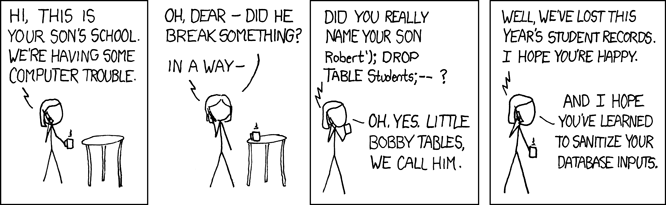
\includegraphics[width=0.7\textwidth]{images/exploits_of_a_mom}\\
Obligatory XKCD ( \url{https://xkcd.com/327/} ).
\end{center}

\subsection*{Triggers}

It is possible to define an operation in the database that will take place automatically when some other modification of the database takes place. As you might imagine from the name, it follows a logic of ``if x happens, then do y''. 

To define a trigger we need to define~\cite{dsc}:
\begin{itemize}
	\item An event that causes the trigger to be checked.
	\item A condition that must be satisfied for actions to be taken.
	\item The actions to be taken.
\end{itemize}

Triggers are useful in a few scenarios. They can be used to cause some events to occur such as updating related data, checking an integrity constraint that would be too difficult to check any other way, or alerting humans that some condition is satisfied. I generally discourage the first use: application logic should probably be the one that modifies the data. Checking integrity is a good use. Alerting humans is usually something like sending an email... No program is complete unless it sends e-mail.



\bibliographystyle{alphaurl}
\bibliography{356}


\end{document}
